
\subsection{Fuzzy C-Means}

We have tested 432 different configurations of the Fuzzy C-Means (FCM) algorithm on each dataset by using the fuzziness parameter \( m \) (with values from 1.5 to 4.0) and varying the number of clusters ( n\_clusters) between the following values:

\begin{itemize}
  \item Pen-based: 6, 8, 9, 10
  \item Mushroom and Hepatitis: 2, 3, 4, 5
\end{itemize}


The following parameters were also varied:


\begin{itemize}
  \item \( \text{max\_iter} \): 100, 300, 500
  \item \( \text{error} \): 1e-1, 1e-4, 1e-5
  \item \( \rho \): 0.5, 0.7, 0.9
\end{itemize}


For each configuration, we ran the algorithm 10 times to mitigate the effects of initialization randomness, resulting in a total of 4320 runs of the FCM algorithm per dataset. From the evaluation metrics extracted in these runs, we analyze the impact of the key hyperparameters and derive insights through statistical analysis.

We decided not to include \textit{max\_iter} and \textit{error tolerance} in the analysis of performance metrics, as they do not significantly affect the performance, aside from removing outliers and slightly improving execution time. To illustrate this, we include 3 heatmaps displaying execution times for each dataset, along with the distribution of ARI results for different values of \textit{max\_iter} and \textit{error tolerance} (see \textbf{Figure}\ref{fig:error-iter-fuzzy}).


\begin{figure}[H]
    \centering
    \begin{subfigure}{0.32\textwidth}
        \centering
        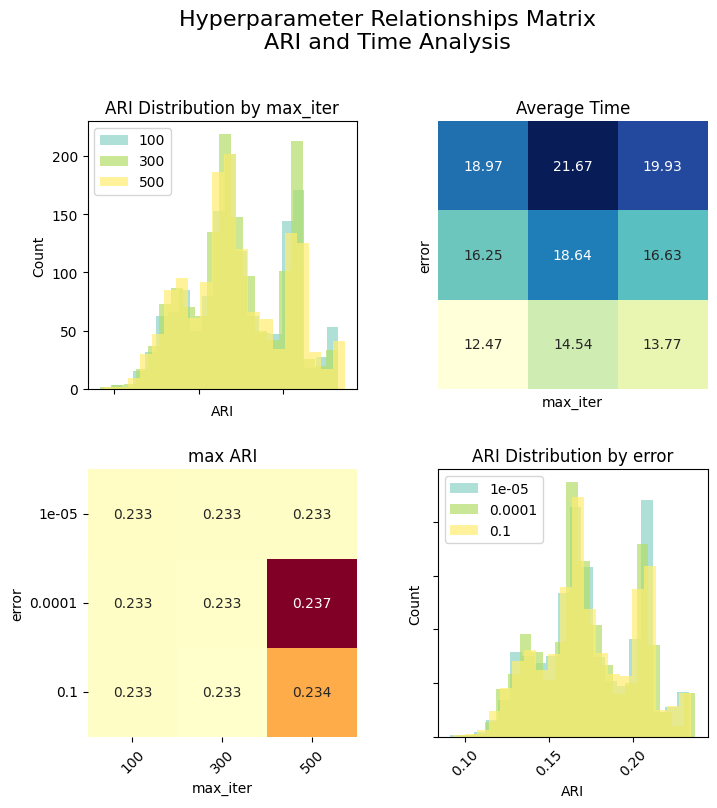
\includegraphics[width=\linewidth]{figures/FuzzyCMeans/penBased_error_iter_pairplot.png}
        \caption{Pen-based dataset.}
    \end{subfigure}
    \begin{subfigure}{0.32\textwidth}
        \centering
        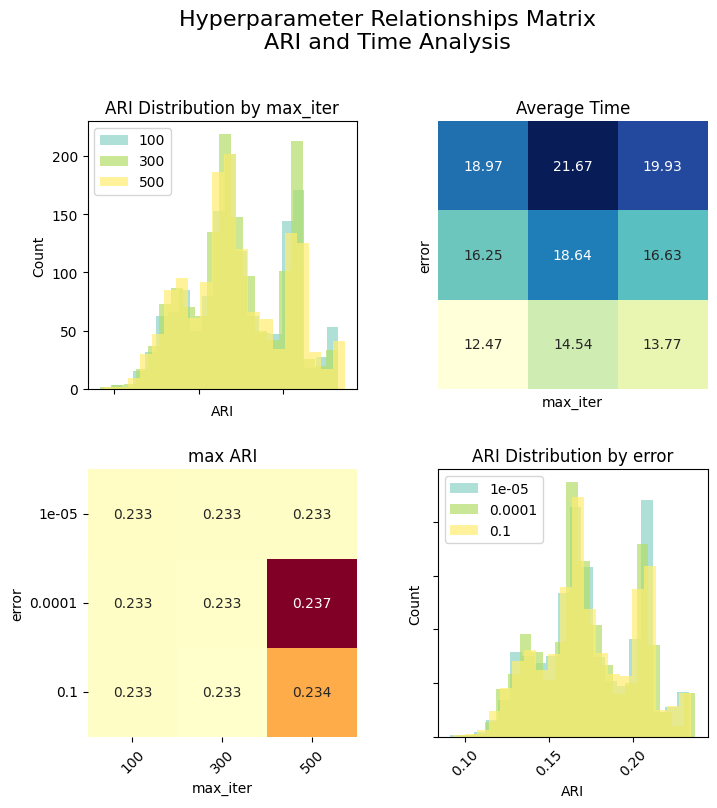
\includegraphics[width=\linewidth]{figures/FuzzyCMeans/mushroom_error_iter_pairplot.png}
        \caption{Mushroom dataset.}
    \end{subfigure}
    \begin{subfigure}{0.32\textwidth}
        \centering
        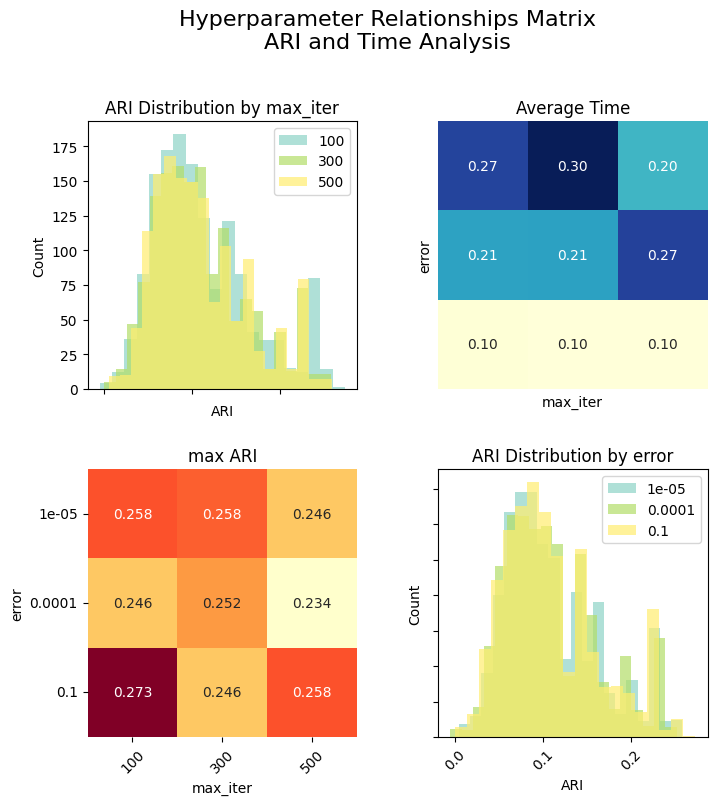
\includegraphics[width=\linewidth]{figures/FuzzyCMeans/hepatitis_error_iter_pairplot}
        \caption{Hepatitis dataset.}
    \end{subfigure}
    \caption{Heatmaps illustrating execution times for each dataset, showcasing performance across different configurations.}
    \label{fig:error-iter-fuzzy}
\end{figure}


\subsubsection{Preliminary Study}

We first explored preliminary patterns in the measured metrics and the influence of hyperparameters on clustering performance.


\textbf{Figure} \ref{fig:metrics_corr_fuzzy} illustrates the relationships between the various metrics for the FCM algorithm. This matrix plot highlights the correlations between metrics (lower triangle), histogram distributions (diagonal), and scatterplots of metric values (upper triangle). A notable observation is the interaction between the fuzziness parameter and metrics like Silhouette and DBI. For instance, while lower fuzziness (mm) often improves silhouette scores due to sharper cluster boundaries, it can lead to higher DBI values, which might indicate a trade-off between cluster compactness and interpretability. Similar trends are observed across all datasets, though the degree of correlation varies.


\begin{figure}[H]
	\centering
	\begin{subfigure}{0.32\textwidth}
		\centering
		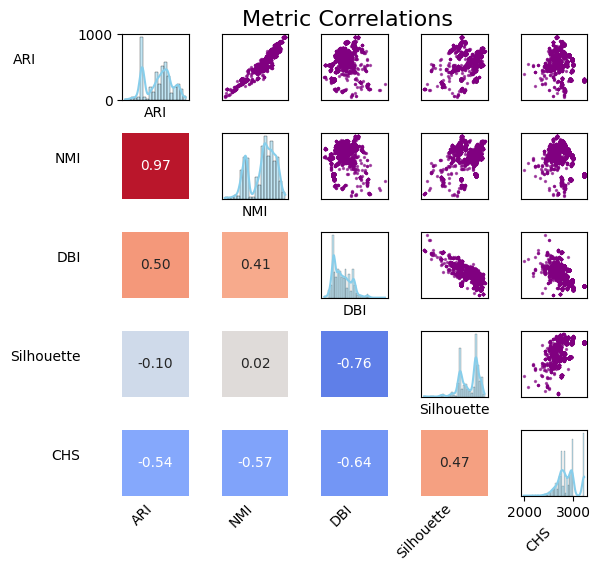
\includegraphics[width=\linewidth]{figures/FuzzyCMeans/penBased_metrics_correlations_matrix.png}
		\caption{Pen-based dataset.}
	\end{subfigure}
	\begin{subfigure}{0.32\textwidth}
		\centering
		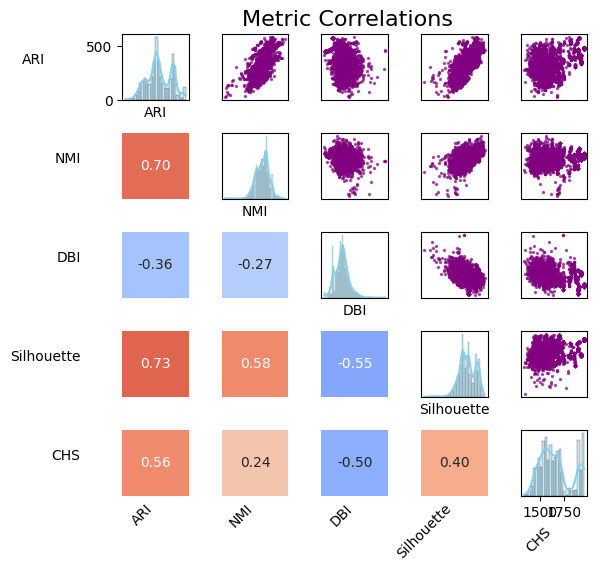
\includegraphics[width=\linewidth]{figures/FuzzyCMeans/mushroom_metrics_correlations_matrix.png}
		\caption{Mushroom dataset.}
	\end{subfigure}
	\begin{subfigure}{0.32\textwidth}
		\centering
		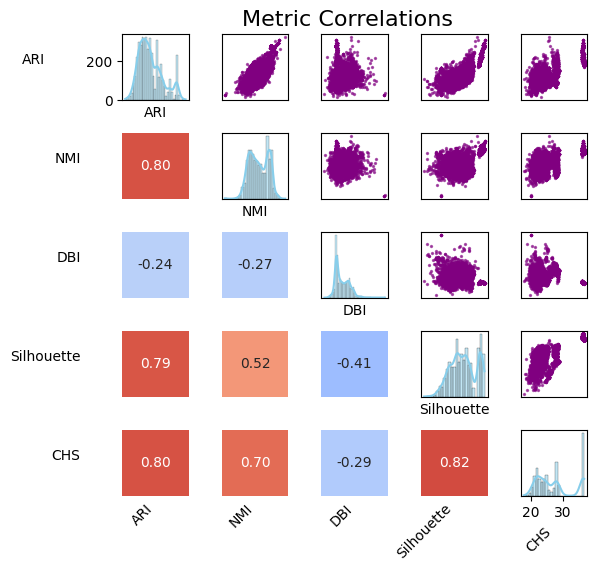
\includegraphics[width=\linewidth]{figures/FuzzyCMeans/hepatitis_metrics_correlations_matrix.png}
		\caption{Hepatitis dataset.}
	\end{subfigure}
	\caption{Metrics correlation acrross the three datasets.}
	\label{fig:metrics_corr_fuzzy}
\end{figure}


Additionally, Figure \ref{fig:pairplot_fuzzy} shows hyperparameter pairwise relationships, particularly the impact of fuzziness $m$ and number of clusters n\_clusters on clustering quality and execution time. Across datasets, higher fuzziness values consistently resulted in more computationally expensive runs, likely due to the increased complexity of assigning membership values. Interestingly, for datasets like Pen-based (10 classes), high cluster counts (e.g., n\_clusters$=10$) aligned closely with ground truth and yielded better metrics, such as ARI and NMI. Conversely, for Mushroom (2 classes), smaller values of n\_clusters and lower fuzziness performed better.


\begin{figure}[H]
\centering
\begin{subfigure}{0.49\textwidth}
\centering
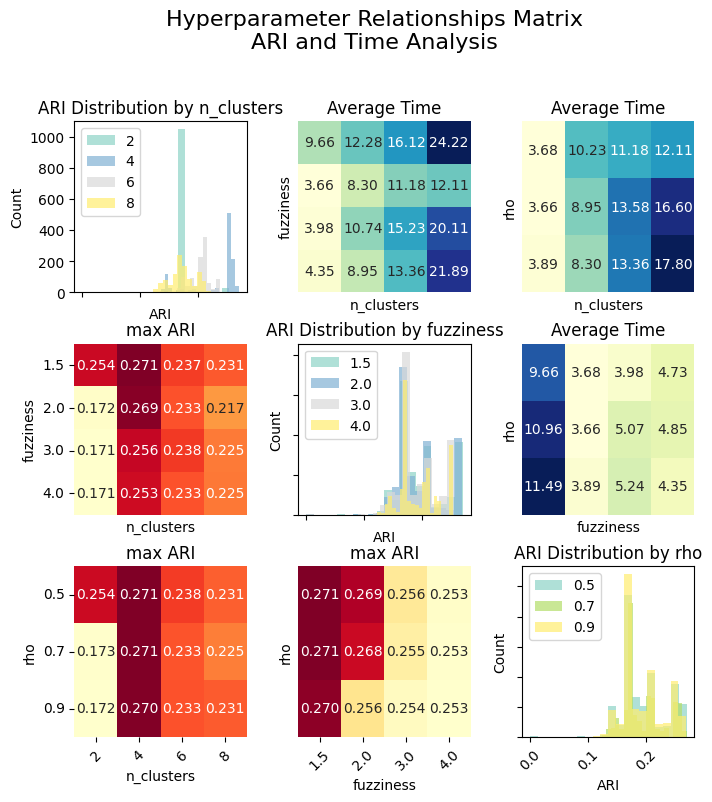
\includegraphics[width=\linewidth]{figures/FuzzyCMeans/mushroom_hyperparameter_pairplot_matrix.png}
\caption{Mushroom pairplot matrix for FCM}
\end{subfigure}
\hfill
\begin{subfigure}{0.49\textwidth}
\centering
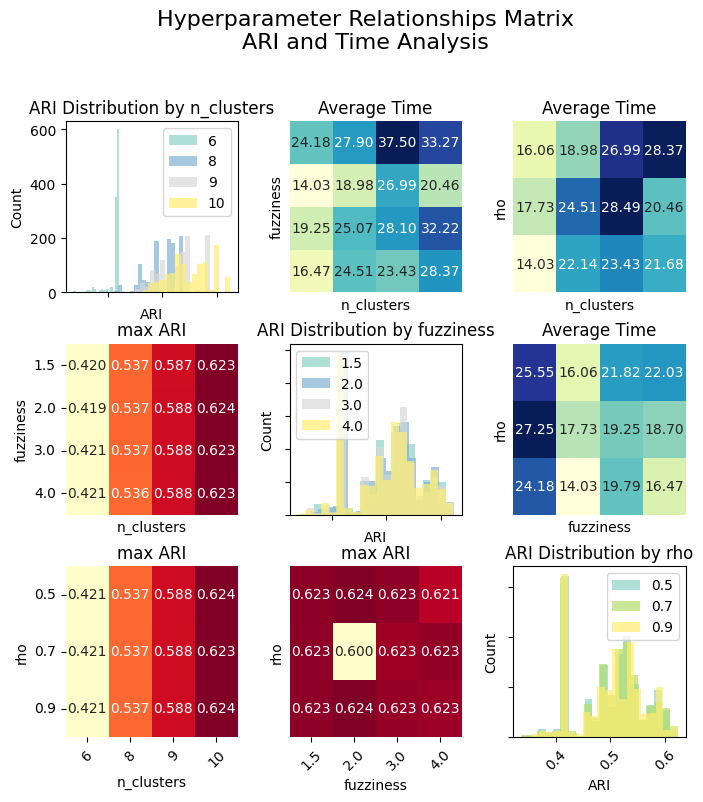
\includegraphics[width=\linewidth]{figures/FuzzyCMeans/penBased_hyperparameter_pairplot_matrix.png}
\caption{Pen-based pairplot matrix for FCM}
\end{subfigure}
\caption{Hyperparameter pairplot matrices based on clustering metrics and execution time for FCM}
\label{fig:pairplot_fuzzy}
\end{figure}



\subsubsection{Fuzziness Parameter (m):}

\begin{figure}[H]
	\centering
	\begin{subfigure}{0.32\textwidth}
		\centering
		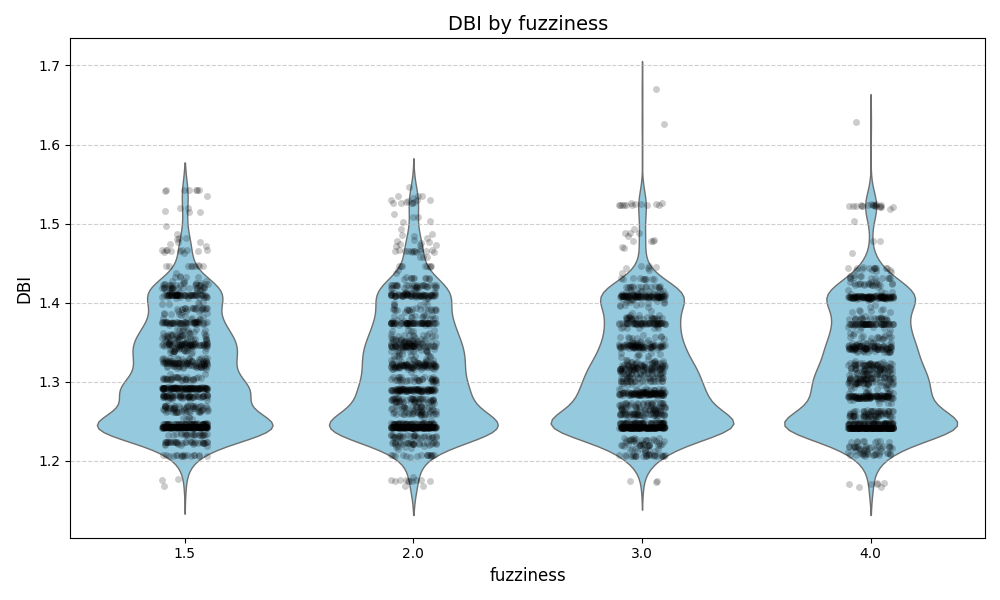
\includegraphics[width=\linewidth]{figures/FuzzyCMeans/penBased_violin_fuzziness_vs_DBI}
		\caption{Pen-based dataset.}
	\end{subfigure}
	\begin{subfigure}{0.32\textwidth}
		\centering
		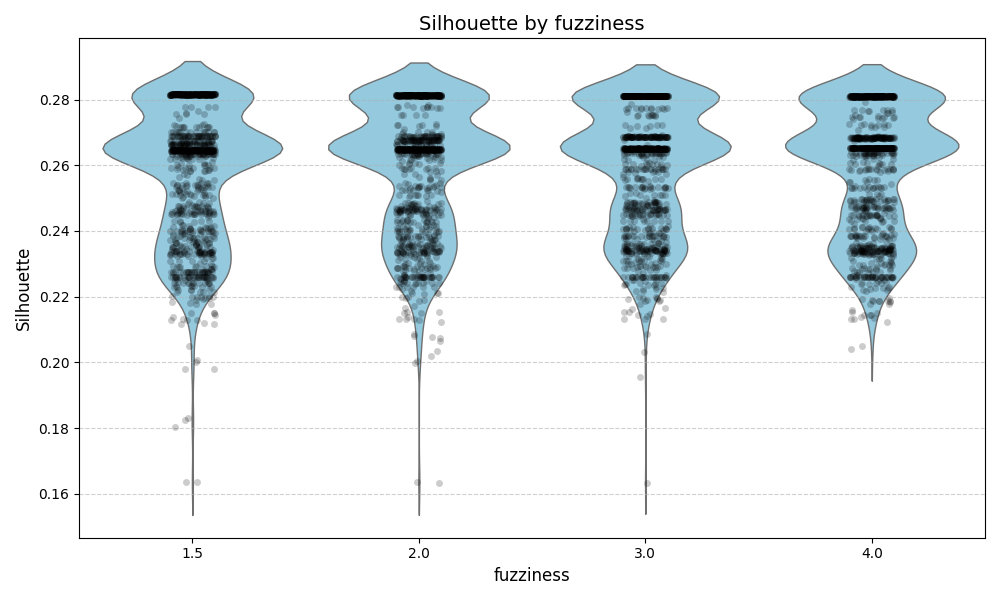
\includegraphics[width=\linewidth]{figures/FuzzyCMeans/mushroom_violin_fuzziness_vs_Silhouette}
		\caption{Mushroom dataset.}
	\end{subfigure}
	\begin{subfigure}{0.32\textwidth}
		\centering
		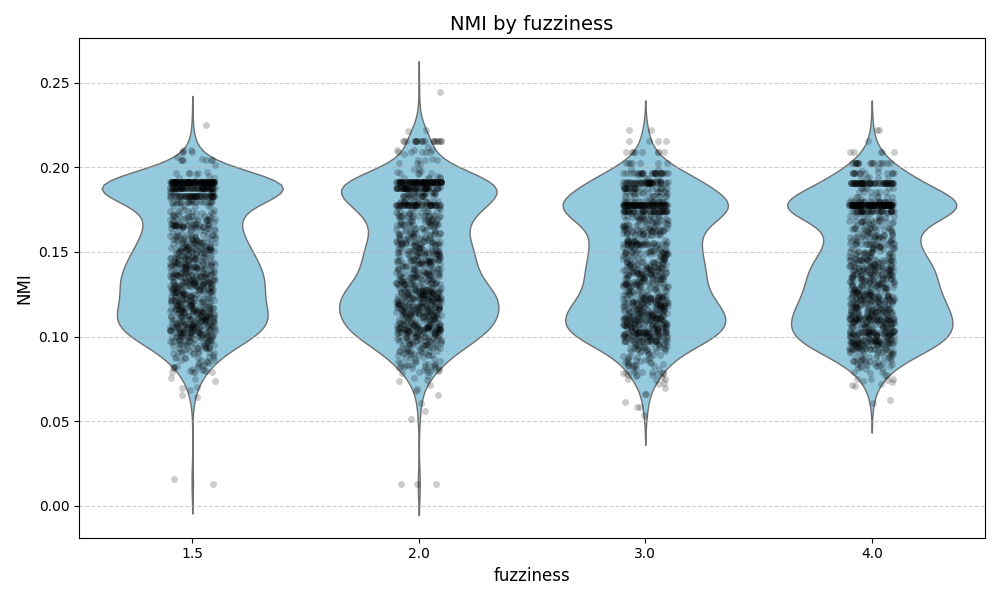
\includegraphics[width=\linewidth]{figures/FuzzyCMeans/hepatitis_violin_fuzziness_vs_NMI}
		\caption{Hepatitis dataset.}
	\end{subfigure}
	\caption{Metrics correlation acrross the three datasets.}
	\label{fig:metrics_corr_fuzzy}
\end{figure}



\begin{comment}
\subsubsection*{Number of Clusters (n\_clusters):}

\begin{enumerate}

\item Hepatitis: Lower cluster counts (e.g., n_clusters=2n\_clusters = 2) showed better ARI and Silhouette scores, aligning with the dataset's two-class structure.

\item Mushroom: Metrics like CHS favored smaller cluster counts, with n_clusters∈[2,4]n\_clusters \in [2, 4] achieving the best results. Silhouette scores corroborated these findings.

\item Pen-based: Higher cluster counts (n_clusters=10n\_clusters = 10) aligned with the dataset's class structure and yielded optimal ARI and NMI. Lower counts led to poor clustering quality, while overly high values showed diminishing returns.

\end{enumerate}

These findings confirm the sensitivity of FCM to both hyperparameters and its suitability for datasets with well-defined class structures.



\subsection*{Highlights from Tables}

\begin{itemize}

\item Pen-based Dataset: Optimal ARI (0.6242) and NMI (0.7073) achieved with n_clusters=10n\_clusters = 10 and m=2.0m = 2.0, reflecting its 10-class nature.

\item Mushroom Dataset: CHS (1962.91) supports n_clusters=6n\_clusters = 6 and m=1.5m = 1.5, showcasing the importance of small cluster counts in this two-class dataset.

\item Hepatitis Dataset: Lower n_clustersn\_clusters and fuzziness values provide better interpretability, with the highest ARI (0.1389) for m=1.5m = 1.5.

\end{itemize}

This adaptation integrates Fuzzy C-Means characteristics while maintaining your original narrative structure.
\end{comment}
